\chapter{Introduction}
\index{Introduction@\emph{Introduction}}%

%\section{blah}
%\index{blah@\emph{blah}}%
%
%\texttt{asdf}
%
%\begin{quote}
%\index{guarantee}%
%This template package is provided and licensed ``as is'' without warranty
%of any kind, either expressed or implied, including, but not limited to,
%the implied warranties of merchantability and fitness for a particular
%purpose. Yadda, yadda, yadda, \ldots
%\end{quote}

This report is a case study of using W3C Web Components, 
\index{Web Components}
a proposed HTML5 extension,
to implement techniques of encapsulation, abstraction, modularity in web application engineering.
The author designed Speakur, a real-time discussion social plugin for the web, 
as an experiment to determine the viability and maturity of using Web Components to create modern, highly composable web applications. Figure~\ref{f:demo1} shows an example of a Speakur discussion.

Like most web applications Speakur is written in a combination of HTML markup and the Java\-script programming language. 
HTML is a declarative markup language used to create documents --- web pages --- which are viewed with the help of a program called the browser. 
The Hyper\-text Markup Language (HTML) 
\index{HTML}
standard has proven wildly successful since its introduction in 1993 by British computer scientist 
Tim Berners-Lee, 
\index{Tim Berners-Lee}
with billions and billions of pages served, 
and hundreds of millions of public and private web sites forming a major part of our information landscape~\cite{internetlivestats.com2015}.
More than any other invention, other than perhaps email, the World Wide Web (WWW) has shaped how we see and use the global network.

% 
\begin{figure}[htb]
\centering
 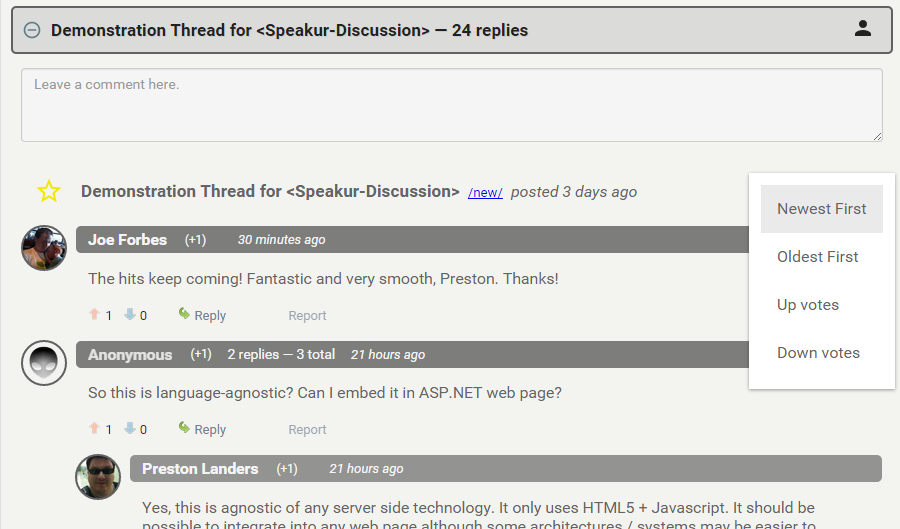
\includegraphics[width=6in]{images/screenshot_20150312_1630_v2.png}
\caption{A Speakur thread inside a demonstration page.}
\label{f:demo1}
\end{figure}
\index{commands!environments!figure}%

Those designing and programming applications for the Web as a computing platform have long dreamed of the ability to mix and match independent, reusable chunks of functionality --- components --- in their documents without mutual coupling and interference. 
The original and current Document Object Model (DOM)
\index{DOM}
browser abstraction provided by HTML does not allow for significant decoupling; 
everything lives together on one big page. Hacks like the 
\tcode{<iframe>} 
\index{iframe}
tag let you work around some of these restrictions, usually in a limited and inelegant way.

At the time of HTML's introduction the concept of quickly and easily composing a static web page, 
much less a full-fledged dynamic application, 
out of Lego-like reusable building blocks seemed like a distant dream at best. 
The introduction of the 
Javascript\footnote{Javascript, also rendered as JavaScript or JS, 
has no significant relation to Sun's (now Oracle's) popular Java\index{Java} programming language;
the name is an unfortunate coincidence at best.

To complicate the naming situation even further, Javascript is officially standardized under the name ECMAScript (ES)\index{ECMAScript}.}
\index{Javascript}
(JS)\index{Javascript} programming language to web browsers in 1995 allowed for a completely new dimension of dynamic behavior that was not possible before~\cite{w3ccontributors2012}.
Eventually web apps like Gmail\index{GMail} and Google Docs\index{Google Docs}, powered by Javascript, rivaled traditional desktop applications in functionality and usability while being instantly accessible from nearly anywhere.
Still, web apps had to be stitched together `by hand' in ways that carefully ensured the different parts didn't step on each other's toes, else disaster frequently ensued. 
Each component or area of the system could not help but be coupled to the others at some level as a result of the programming model imposed by the DOM\index{DOM} and HTML~\cite{ihrig2012}.

Over the years the dynamic behaviors afforded by Javascript grew in importance along with the web, and helped contribute to its success. 
The flexible, loosely typed nature of Javascript aided the prototyping and initial development process,
but the difficulties of building a large application in the DOM soon became apparent.
Over time, a bewildering array of frameworks and libraries sprang up around the HTML/JS ecosystem to help manage this complexity and to provide scaffolding and structure for the client side of web apps.
For many years individual JS frameworks seemed to come and go as ephemerally as teenage pop idols~\cite{allenpike2015}. 
Interoperability between these completing frameworks was virtually non-existent; 
components from one framework typically couldn't be easily combined with those from an another.
The industry kept searching for the Next Big Thing that would make writing high quality web apps less of bug-ridden, messy chore~\cite{allenpike2015}. 

In recent years (roughly 2011 to 2014) Google's Angular~\cite{googledevelopers2015-b}
\index{Angular}
has emerged as a dominant client framework, 
due in part to its high perceived quality~\cite{dickey2014} and the fact that it represents an common point for a fragmented industry to rally around.
Facebook's React~\cite{reactcontributors2015}
\index{React}
JS library with its Virtual DOM is an up-and-comer focused on high performance that is more complementary in nature to Angular than a true challenger.

Yet despite the emergence of the updated HTML5 standard in 2011 and the recent successes of web frameworks like Angular and React in capturing developer attention, 
a clear picture still did not exist of how web apps could achieve the encapsulated component model that had become prevalent in other areas of software engineering.
That is, until engineers from Google\footnote{
As of March 2015, Google's Chrome browser is the most popular desktop browser~\cite{zachte2015}.}
\index{Google}
and Mozilla\footnote{
The Mozilla Foundation is the sponsor of the popular Firefox web browser. It grew out of Netscape, whose Navigator browser helped bring the web to a mass audience.}
\index{Mozilla} 
and other organizations got together in 2012 under a W3C Web Applications Working Group~\cite{w3c2015} 
to draft a new standard called \textbf{Web Components} that will extend and enhance HTML5 in ways that could have a significant long-term impact~\cite{yveslafon2015}. 
For example, as of the time of this writing, a rewrite of Angular called Angular 2.0 is slated to include Web Components as a core architectural element~\cite{santiagoesteva2015}.

\section{Web Components Overview}
Fundamentally, the Web Components standard consists of four new core DOM technologies --- extensions to the current HTML5\index{HTML5} standard.
If these standards are accepted by major browser vendors and the World Wide Web Consortium (W3C)
\index{W3C}
which maintains HTML, 
they will eventually become native browser features and available directly to any web page without needing to use any additional JS frameworks or libraries. 
The core Web Component technologies are~\cite{penades2015}:
\begin{itemize}
\item
\textbf{Custom Elements}\index{Custom Elements}: extending HTML with author-created tags
\item
\textbf{Shadow DOM}\index{Shadow DOM}: encapsulation for the internals of custom elements
\item
\textbf{Templates}\index{Templates}: scaffolding for instantiating blocks of HTML from inert templates
\item
\textbf{Imports}\index{Imports}: packaging for HTML components
\end{itemize}

This report also explores several related web standards initiatives that are frequently associated with Web Components 
but are not formally grouped under them, including mutation observers,
\index{mutation observers}
model driven views, 
\index{model driven views}
and the CSS Flexible Boxes
\index{Flex box} 
and CSS Grid
\index{CSS Grid}
systems. 
In part because many of these technologies are not yet formally accepted as W3C standards and are not yet widely implemented in typical mobile and desktop browsers, 
Speakur has been implemented using Google's experimental Polymer framework~\cite{polymercontributors2015}.\index{Polymer}
Polymer provides a Javascript `polyfill'
\index{polyfill}
library to implement many of the new Web Component features in browsers which would otherwise not support them. 
Eventually this platform polyfill should become unnecessary, in theory, as WC becomes widely adopted in browsers.
Some browsers like Google Chrome 
\index{Google Chrome}
already have at least some native Web Component support and on these browsers the polyfill is effectively a `no-op'.

The potential componentization of the web is one of the most exciting developments in web engineering in years and follows the overall growth in software-as-a-service (SaaS) 
\index{SaaS}
and the service oriented architecture
\index{Service Oriented Architecture}
model. 
The conversion of dynamic web logic---not mere snippets of plain HTML---into bundles of reusable, extendable, composable components enables web developers to move to a higher level of abstraction than was previously possible.

The move towards a component-based Web will enable interesting new composite services, mashups, and may help broaden the potential pool of web developers. 
What previously required a highly integrated, high-overhead development model or lots of tedious glue code can become as simple as importing a custom element and dropping it onto a page.


\section{Structure of This Report}
\index{Structure of This Report@\emph{Structure of This Report}}%

The goal of this report is to demonstrate the application of software engineering design patterns embodied in the W3C proposed Web Components standard such as encapsulation, modular composition, and the synchronization of distributed application state. 
This report discusses many of the goals and principles of the Web Components initiative and how a number of different technologies taken together help raise the overall level of abstraction for content authors, web engineers, and application developers --- which I will refer to collectively as (web) authors for short.

The Background section provides an introduction to some of the architectural problems inherent in modern web authoring and how Web Components (WC) address them. 
It also provides some background the on software engineering design patterns that are embodied in Web Components such as encapsulation and composition.
It describes some of the motivations behind the development of Speakur and some of the specific software engineering questions it addresses, such as the ability to provide a hassle-free way to host an embedded discussion forum inside an arbitrary web resource in a way that is fully encapsulated.

The Approach section describes the high level software architecture choices behind Speakur and details the specific structures and techniques used when constructing a Web Component.
It describes how Speakur uses WC to implement encapsulated modules whose internals are protected from unintentional outside influence. 
It also describes how the choice of the Firebase cloud database service and its Websocket-based event notification system impacts Speakur's architecture.

The Implementation section shows how to apply Web Component principles to the task of creating a flexible and generic discussion forum for both desktop and mobile browsers. 
It describes the low level architecture, code flow, and synchronization process.
An important topic in this section is security: how can we implement a largely client-based system while maintaining some kind of data integrity?

This is followed by an Analysis section which discusses some of the outcomes as compared to the original goals and also looks at the impact of the selection of Web Components, Polymer, Firebase and some of the other architectural choices. 
A few quantitative results are included, I hope \textbf{(TODO)}.

Finally, the Conclusion section is there and wraps up the report with various words \textbf{(TODO)}. 

\section{Source Code and Demonstration Resources}
\index{Source Code and Demonstration Resources@\emph{Source Code and Demonstration Resources}}%

The source code for Speakur consists of HTML\index{HTML} and Javascript\index{Javascript} files located in a Git\index{Git} version control repository. 
These files constitute an ``HTML Import''\index{HTML Imports} package that provides a
\textbf{\tcode{<speakur-discussion>}}
custom HTML element\index{Custom Element} for the use of web authors in their own pages.
An example of using \tcode{<speakur-discussion>} is given in Chapter 3 and in briefly in Listing~\ref{example1} below.

\begin{lstlisting}[language=HTML5,numbers=none,caption=
{Example of the Speakur custom HTML element},label=example1,captionpos=below]
 <!-- place this on your page
      where you want a discussion -->
 <speakur-discussion
   href="http://example.com/news/web-components-in-action"
   allowAnonymous="false">
 </speakur-discussion>
\end{lstlisting}

The Speakur source code and component documentation can be found on the social coding site GitHub.com at~\cite{landers2015-b}:

\tcode{\url{https://github.com/Preston-Landers/speakur-discussion}}

Demonstrations of several web pages which show off embedded Speakur discussions are available at the following location~\cite{landers2015-c}:

\tcode{\url{https://preston-landers.github.io/speakur-discussion/components/speakur-discussion/demo.html}}
